\chapter{Antecedentes}%\selectlanguage{spanish}

% BAGOTSKY book has good information on the lithiuom ion batteries, talks about intercalation and mentions oxidation states changes in cathode metals during charge or discharge

% https://sci-hub.tw/10.1016/j.resconrec.2016.07.002

%https://www.sciencenews.org/article/search-new-geologic-sources-lithium-could-power-clean-future

\section{El litio como un elemento estratégico}
El litio es un elemento clave para sectores económicos de gran importancia, ya que, sus propiedades hacen de él y de algunos de sus compuestos, muy adecuados para diferentes aplicaciones. En dispositivos de almacenamiento de energía eléctrica son útiles su extremo potencial estándar de reducción (-3.045~V, el menor para los elementos de la tabla periódica) y su baja masa atómica, que le provee una excelente relación carga/masa \citep{Bagotsky2006}. Tiene la capacidad calorífica específica más alta de los elementos sólidos (3.489~J~mol\mnn\ a 20$^o$C), y un muy alto coeficiente de expansión térmica, por lo que provee resistencia a cerámicos y vidrios frente a cambios bruscos de temperatura \citep{Hart1973}. El litio también es utilizado ampliamente en la elaboración de grasas y lubricantes especiales (en forma de sales líticas de ésteres de ácidos grasos), en producción de aluminio aeroespacial (para lo que se usa litio metálico de elevada pureza), en la elaboración de polvos fundentes, y en la deshumidificación de aire.

\begin{figure}[htbp]
    \subbottom{\begin{picture}(500,210)
               \put(5, 0){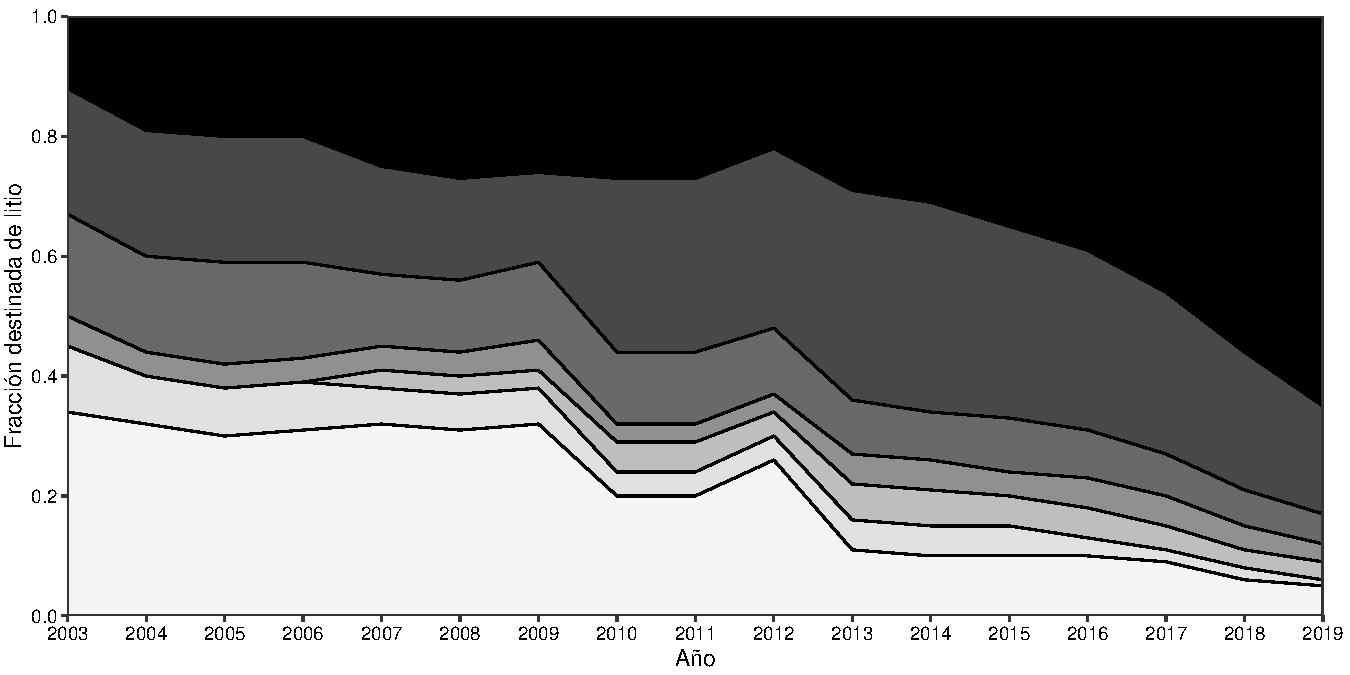
\includegraphics[width=0.986\textwidth,trim={0 0.85cm 0 0}, clip]{chap2/images/usesRel.pdf}}
               \put(2, 202){\large a)}
               \end{picture}}\\%
    \subbottom{\begin{picture}(500,230)
               \put(0, 0){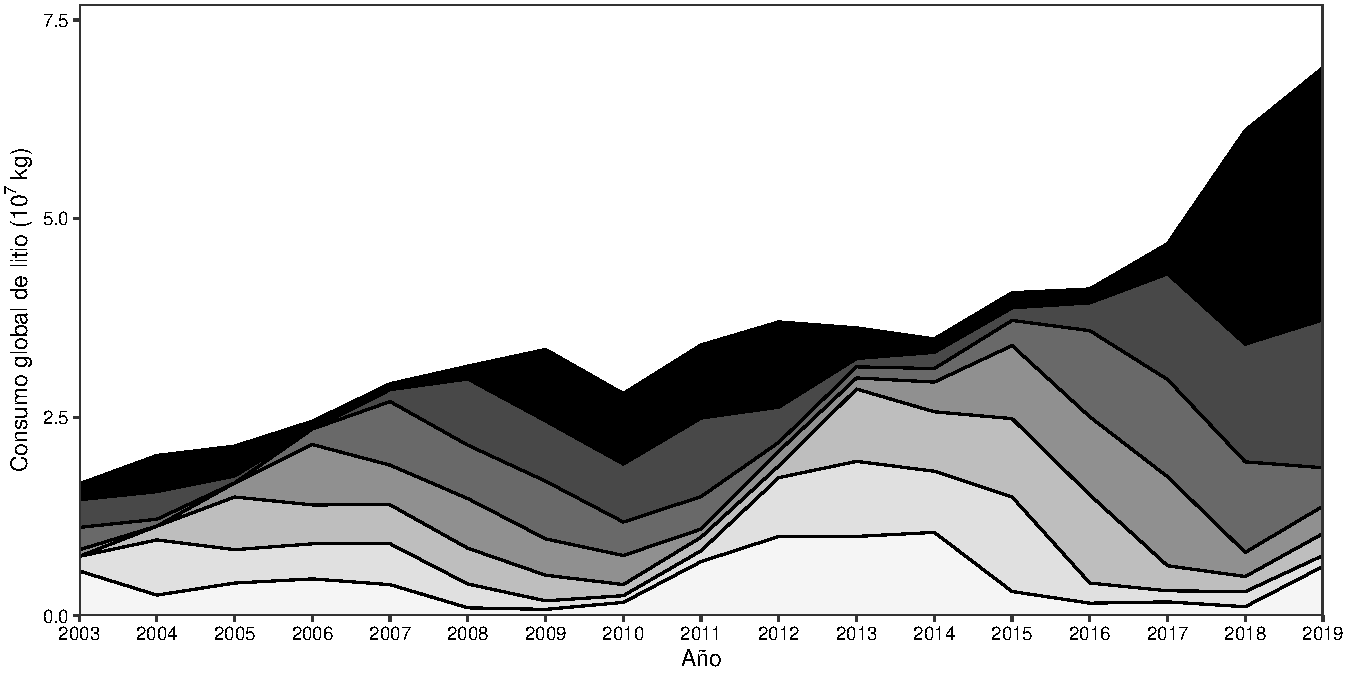
\includegraphics[width = \textwidth]{chap2/images/usesAbs.pdf}}
               \put(0, 223){\large b)}
               \end{picture}}
    \caption[Series de tiempo mercados finales de consumo de litio desde el año 2003.]{Mercados finales de consumo de litio desde el año 2003. (a) en proporción y (b) en cantidades absolutas. Las zonas del gris más oscuro al más claro corresponden a fabricación de baterías, mejoramiento de cerámicos y vidrios, fabricación de lubricantes, síntesis de polímeros, elaboración de polvos fundentes, tratamiento de aire, y otros usos (aleaciones con aluminio, uso farmacéutico, entre otros) respectivamente.  Elaborado con datos recolectados de \citet{    SQM2003, SQM2004, SQM2005, SQM2006, SQM2007, SQM2008, SQM2009, USGS2011, USGS2012, USGS2013, USGS2014, USGS2015, USGS2016, USGS2017, USGS2018, USGS2019}.}
    \label{fig:uses}
\end{figure}

La Figura \ref{fig:uses} contiene la serie de tiempo de la evolución del mercado final del litio producido en el mundo desde el año 2003. El mercado de baterías ha monopolizado más del 60\% del consumo global de litio, que solía estar distribuido más o menos con uniformidad entre diversas industrias. En la figura con escala absoluta (Figura \ref{fig:uses}(b)), puede observarse que en los últimos años la demanda de este sector aumenta casi constantemente. Esto responde al uso cada vez más dispositivos portátiles, que por lo general funcionan con energía almacenada en baterías de ion de litio \acused{LIB}(LIBs) y, principalmente, al mercado de los vehículos eléctricos \acused{EV}(EVs) que cada vez gana más protagonismo en medio de la tendencia global hacia la utilización de energías y tecnologías más limpias desde un punto de vista ambiental. Adicionalmente, en algunos escenarios se especula que las baterías con litio serán la opción predilecta para almacenar energía eléctrica proveniente de fuentes renovables cuando la quema de combustibles fósiles se haga obsoleta \citep{SVERDRUP2016}.

La relevancia de este elemento ha sido reconocida por organismos gubernamentales de distintos países. La Dirección General de Desarrollo Minero de la \citet{SecEc2018} habla de la importancia de este elemento, y menciona algunos de los potenciales yacimientos que podrían posicionar al país como una potencia mundial de este recurso. El Servicio Geológico de Estados Unidos (USGS) considera que el litio es un elemento crítico que podría hacer contribuciones importantes hacia la tan anhelada autonomía energética de ese país \citep{Bradley2017}. El Servicio Geológico Británico considera al litio en su \textit{lista de riesgo} de suministro de elementos y lo ubica al mismo nivel de importancia que los metales preciosos del grupo del platino \citep{STERBA2019416}. La Unión Europea no considera al litio como un elemento crítico, pero admite que su importancia crece constantemente \citep{European2018}.

El suministro mundial de litio puede ser suficiente para varias décadas por venir, pero su futuro encarecimiento y escasez es inevitable si la flota automotriz es reemplazada en su totalidad por vehículos de propulsión eléctrica \citep{SVERDRUP2016}. Una gran parte de los análisis prospectivos que abordan la dinámica de la demanda y la oferta de metales críticos para las próximas décadas, centran su atención al caso del litio incluso a expensas de que algunos otros metales, considerados como más críticos, están siendo ignorados en gran medida \citep{Watari2020}. Si la oferta mundial de litio llega a ser incapaz de satisfacer las necesidades del creciente sector transporte, se ralentizaría la migración masiva de este sector hacia el uso de energías más limpias \citep{VIKSTROM2013}. Algunos autores concluyen que en un futuro cercano el litio no es un cuello de botella para el suministro de las materias primas necesarias para la fabricación de \acp{LIB}, pero esto podría modificarse drásticamente obedeciendo cambios políticos o económicos que incentiven un crecimiento inesperado del sector de transporte eléctrico \citep{Olivetti2017}. En efecto, varios factores aceleran hoy por hoy el crecimiento de este sector. Un ejemplo radical lo presenta el Reino Unido de Gran Bretaña e Irlanda del Norte, cuyo gobierno ha impuesto un veto a la venta de vehículos de combustión e híbridos para el año 2035, y un veto a su circulación para el año 2050 \citep{BBC2020}.

Las \acp{LIB} son actualmente la mejor tecnología para el almacenamiento de energía eléctrica \citep{Zubi2018}. Su desarrollo entre 1970 y 1985 representó un aporte muy importante, por lo que los científicos John Goodenough, Stanley Whittingham, y Akira Yoshino fueron galardonados con el Premio Nobel de Química en el 2019 por los aportes realizados a su invención \citep{Royal2019}. Hoy en día, medio siglo después de los primeros avances en la materia, la investigación de materiales para la producción de baterías cada vez más robustas y eficientes continúa con ahínco. Por ejemplo, recientemente \citet{Harlow2019} reportaron una nueva \ac{LIB} de muy alto desempeño que podría funcionar en un auto eléctrico durante 1.6\e{6}~km, un orden de magnitud por encima de la longevidad promedio de los automóviles actuales.% Este desarrollo (patrocinado por Tesla Inc., el gigante de los autos eléctricos) ayuda a resolver uno de los mayores inconvenientes relacionados con el sector de la transportación impulsada por energía eléctrica. %\citep{Ford2012}.

% READ THIS!!!
% https://www.nobelprize.org/uploads/2019/10/advanced-chemistryprize2019-2.pdf
\clearpage
\subsection{Contexto geoeconómico}
Como en la mayoría de los elementos de la tabla periódica, la distribución del litio no es uniforme alrededor del mundo. Los mapas de las reservas y los recursos de litio por país se muestran en las Figuras \ref{fig:reservas} y \ref{fig:recursos}, respectivamente. Las reservas hacen alusión a cantidades probadas de un elemento, extraíbles de una manera económicamente viable. Los recursos hacen alusión a la estimación total de un elemento en un determinado territorio. La diferencia entre reservas y recursos viene dictaminada principalmente por la demanda de un elemento, ya que esta afecta el precio al cual se adquieren sus productos \citep{VIKSTROM2013}. 

Los mayores productores de litio actualmente son Australia y Chile. El litio de Australia es extraído de minerales que muchas veces son comercializados en forma de concentrados que requieren procesos cortos de beneficiación. Estos concentrados son usados directamente en la manufactura de cerámicos y vidrios \citep{Bradley2017}. El litio de Chile se encuentra en forma de minerales disueltos en lagos salados (i.e.\ salares).  Bolivia, Argentina y Chile son los países con los recursos de litio más grandes del mundo. Estos países definen el llamado {triángulo del litio} por la vasta cantidad de litio que tienen en sus salares. Mientras la extracción del litio de Bolivia no es viable económicamente hoy por hoy, Argentina es el cuarto productor de litio más importante \citep{USGS2020}. China tiene reservas importantes de litio y es el tercer productor más importante de este elemento. Sin embargo, el gigante asiático depende fuertemente de las importaciones debido a que por su alto nivel de industrialización consume cerca de la mitad del litio producido mundialmente cada año \citep{Olivetti2017}. 

Los recursos de litio más importantes del mundo se encuentran en los océanos, con un volumen total estimado de 1.37\e{9}~km$^3$ y una concentración promedio de ion litio de alrededor de 0.18~mg~kg\mnn\ \citep{KRESS20191, Evans2013, HOSHINO201311}. La cantidad de litio presente en este medio puede ser de alrededor de 250 millones de toneladas. Este valor es mucho mayor que las reservas combinadas de todos los países ricos en litio \citep{Yang2018}. En la actualidad, la extracción de ion litio a partir de agua de mar no es viable económicamente debido a su baja concentración y a la presencia de altos niveles de cationes que interfieren en su proceso de recobro. El costo de extracción de ion litio a partir de agua de mar es el más elevado y se encuentra en el extremo opuesto de una lista encabezada por el Salar de Atacama, en Chile, de donde el kilogramo de carbonato de litio equivalente\acused{LCE} (LCE)\footnote{El carbonato de litio equivalente es la terminología estándar usada en la industria del litio. 1~$kg$ de litio es equivalente a 5.323~$kg$ LCE.} se extrae a menos de 2 dólares estadounidenses (USD)\acused{USD} \citep{KUSHNIR2012}. A pesar de la no viabilidad económica de la extracción del ion litio presente en agua de mar, vale la pena anudar esfuerzos en el desarrollo de nuevas metodologías que permitan su recobro a partir de esta matriz porque hacia allá se puede volcar el mercado de extracción de ion litio cuando sus fuentes continentales, más rentables y menos complicadas, empiecen a escasear.

El precio de los compuestos principales de litio ha aumentado casi constantemente en los últimos años \citep{MARTIN2017}. En el 2019, en medio de la guerra comercial entre China y Estados Unidos, China redujo los generosos subsidios que estaba otorgando a compradores y fabricantes de \acp{EV} y esto produjo una sobreoferta de litio que repercutió en una disminución de su precio en casi un 25\% \citep{Kalantzakos2019}. Sin embargo, la popularidad de los \acp{EV} sigue en aumento, y la balanza de la oferta-demanda podría inclinarse nuevamente a favor de los países productores de litio en cualquier momento \citep{LIU2019}.

%https://sci-hub.tw/10.1016/j.watres.2019.01.050

% https://sci-hub.tw/10.1016/j.apenergy.2013.04.005

\begin{figure}[H]
    \centering
    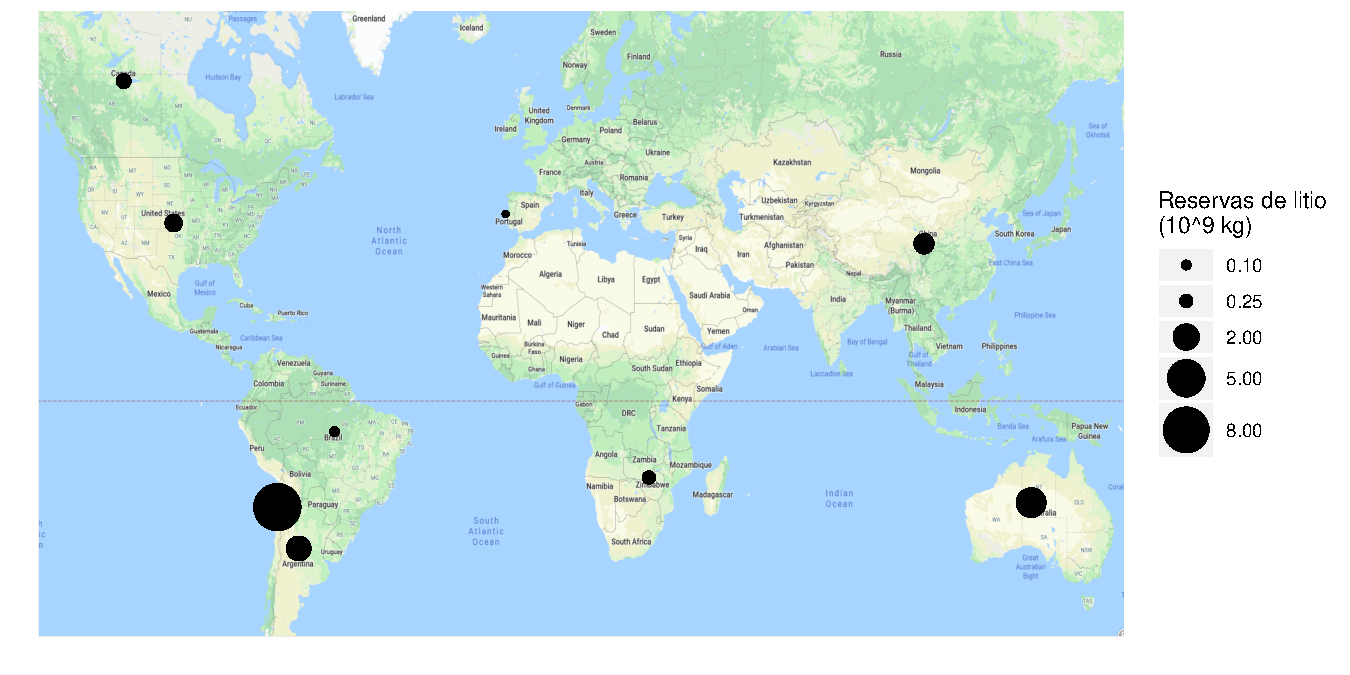
\includegraphics[width = \textwidth, trim = {1cm 1.2cm 0.4cm 0.5cm}, clip]{chap2/images/reserves.pdf}
    \caption[Reservas de litio por país.]{Reservas de litio por país. El diámetro de los círculos es proporcional a la cantidad de litio en millones de toneladas \citep{USGS2020}.}
    \label{fig:reservas}
\end{figure}
\begin{figure}[H]
    \centering
    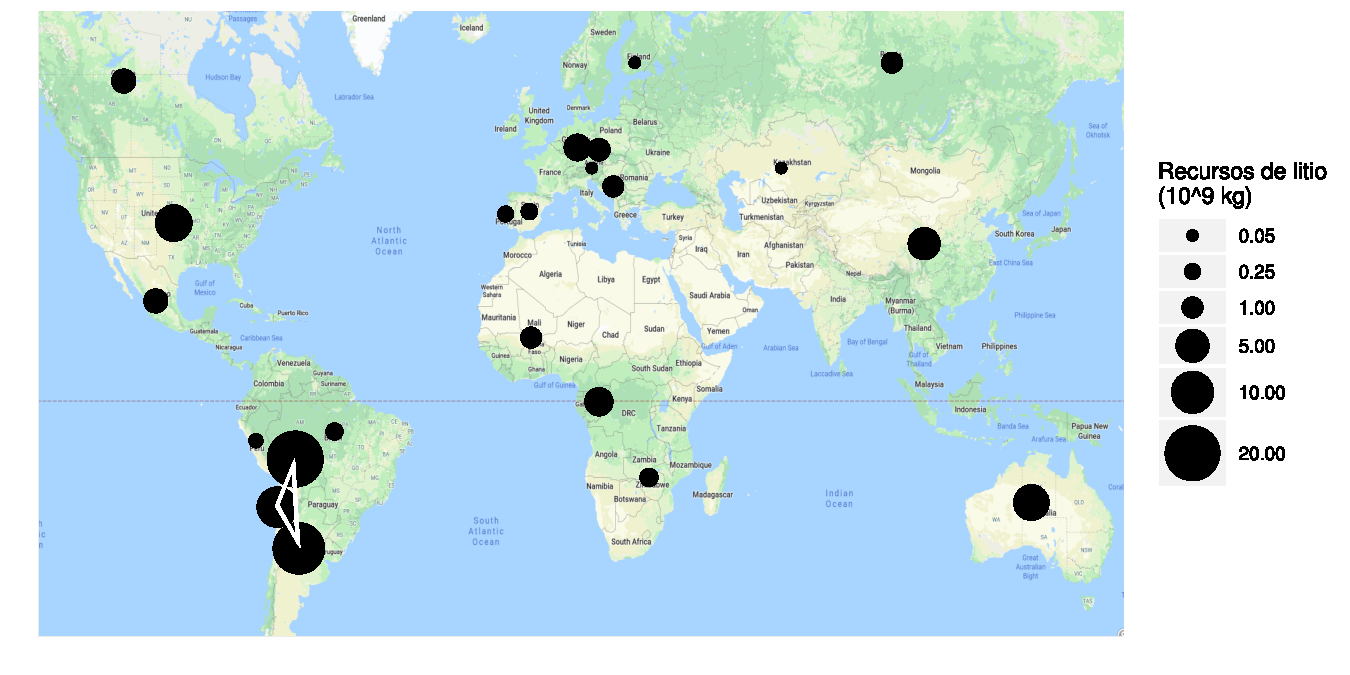
\includegraphics[width = \textwidth, trim = {1cm 1.2cm 0.4cm 0.5cm}, clip]{chap2/images/resources.pdf}
    \caption[Recursos de litio por país.]{Recursos de litio por país. El diámetro de los círculos es proporcional a la cantidad de litio en millones de toneladas \citep{USGS2020}. El {triangulo del litio} en Suramérica se señala con blanco.}
    \label{fig:recursos}
\end{figure}

\subsection{El litio de México}\index{Litio!Bacadéhuachi-Sonora}
%https://www.gob.mx/cms/uploads/attachment/file/419275/Perfil_Litio_2018__T_.pdf
%https://www.bacanoralithium.com/pdfs/Ni-43-101-Mineral-Resource-Estimate-For-The-Sonora-Lithium-Project-Mexico-May-2015.pdf
%https://www.bacanoralithium.com/pdfs/Bacanora-FS-Technical-Report-25-01-2018.pdf
México no figura entre los grandes productores de litio. Como puede observarse en la Figura \ref{fig:reservas}, el Servicio Geológico de Estados Unidos no contabiliza reservas en este país. % y la Figura \ref{fig:recursos} muestra que los recursos que le atribuyeron a México no llegan a las dos millones de toneladas. 
No hay proyectos de extracción de litio en fase de explotación comercial en territorio mexicano y las importaciones de este elemento involucran un negocio multimillonario que se encuentra exento de pagos arancelarios \citep{SecEc2018}. A pesar de esto, en un futuro cercano México podría sentarse en la mesa de las potencias del litio.

Se encuentran en etapa de exploración cerca de 11 proyectos de extracción de ion litio, de los cuales el más importante se encuentra en Bacadéhuachi, en el estado de Sonora, al norte del país. A esta locación se le atribuye ser actualmente el proyecto de explotación de litio más grande del mundo, con una exorbitante cantidad de más de 240 millones de toneladas de mineral con una concentración promedio de litio de 0.35\% en masa \citep{Bacanora2018}. Esta cifra ha sido muy mal utilizada por la prensa común, que irresponsablemente habla de {240 millones de toneladas de litio}.\footnote{Esto es equivalente a la cantidad total de litio presente en la vastedad de los océanos, el mayor reservorio de litio de nuestro planeta.} Esto puede conducir a la errónea conclusión de que México es, como ellos anuncian, la nueva Arabia Saudita del litio. La estimación real en el yacimiento es de cerca de un millón de toneladas extraíbles a un excelente costo total de producción de aproximadamente 4 \ac{USD}~kg$_{LCE}^{-1}$. Estas cifras son bastante prometedoras, y ubican al país como el cuarto o quinto con las mayores reservas de litio en el mundo. El yacimiento consta principalmente de arcilla de hectorita (ver Sección \ref{sec:arcillas}). Ya se encuentra en operación una planta piloto de refinamiento y purificación para la obtención de carbonato de litio de grado para baterías ($\geqslant$99.5\%). Se espera que la mina entre en operación en el 2022 \citep{Bacanora2018}.

% Tesla y Bocanora firmaron convenio para asegurar el suministro de litio al gigante de los EVs

%La zona del yacimiento de litio de Bacadéhuachi-Sonora es actualmente azotada por violencia de los carteles de narcotráfico y se le considera una región inestable. Resulta inevitable rememorar  los yacimientos de oro en el norte del País y el contexto de la fiebre del oro de California en la época de la injusta guerra México-Estados Unidos que cambió tan drásticamente el mapa de Norteamérica. Los tiempos han cambiado desde entonces. Casualmente, el litio ha sido denominado por muchos como oro/petroleo blanco \citep{Crooks2018} y el hecho de que el yacimiento se encuentre \textit{tan lejos de Dios y tan cerca de los Estados Unidos} (a menos de 300 km de la frontera México-Estados Unidos) puede tener poco que ver pues atravesar el océano atlántico no fue inconveniente para los Estados Unidos en el conflicto bélico con (su ex-aliado) Irak en la Segunda Guerra del Golfo para ocupar su territorio y disponer de sus recursos bajo un pretexto que nunca pudo ser demostrado. Sin embargo, una posible invasión suena muy inverosímil y los amados del neoliberalismo tienen herramientas más sutiles para despojar de sus recursos a los países que despectivamente han denominado \textit{tercermundistas}. El Gobierno de México debe pensar al respecto con calma y aparte de recordar siempre su historia para no tener que repetirla, puede aprender de algunos de los muchos errores de su \textit{Aliado del Pacífico},\footnote{La Alianza del Pacífico es un acuerdo de cooperación multilateral establecida en el 2011 por Chile, Colombia, México y Perú. El propósito es prosperar juntos y crear un bloque latinoamericano competitivo frente al mundo \citep{Prado2016}.} el Gobierno Colombiano, y evitar un detrimento irremediable de su Patrimonio Nacional.\footnote{En el año 2000, el Gobierno de Colombia vendió (regaló) su participación en la mina de carbón térmico bituminoso de alta calidad más importante de Latinoamérica, El Cerrejón. El evento coincidió con un alza pronunciada en el valor comercial de este recurso. Mientras en la zona de la mina se presencia pobreza extrema y un medio ambiente sumamente deteriorado, cada 4 horas salen locomotoras con más de $10^7$ kg de carbón que es vendido al mejor postor por parte empresas extranjeras que supieron, en el momento correcto, manipular y comprar a políticos endebles y corruptos que abundan en ese país sudamericano.}


%\subsection{Propiedades químicas}
\subsection{Principales fuentes de ion litio}\index{ion litio!fuentes}
Las principales fuentes de ion litio, sus compuestos más comercializados y el uso más común de los mismos se muestran en la Figura \ref{fig:esquemaSpiers}. Como se mencionó anteriormente, las reservas son fuentes extraíbles con procesos económicamente viables y los recursos incluyen todas las fuentes del elemento a pesar de la inviabilidad práctica de su extracción. A pesar de que el ion litio se encuentra presente en minerales, salmueras, arcillas y (principalmente) en agua de mar, la extracción a gran escala solo se hace actualmente partir de minerales (rocas), y salmueras. Con el éxito de las minas como las de Sonora en México, las arcillas pueden pasar a formar parte importante de las fuentes comerciales de este elemento. Ya se encuentran en operación plantas piloto para la producción de carbonato de litio a partir de arcillas y producen litio a precios muy competitivos \citep{Bacanora2018}.

Los procesos extractivos industriales pueden compartir características generales para fuentes de la misma naturaleza, pero las metodologías aplicables a un determinado yacimiento dependen en gran medida de las particularidades que presentan los recursos de dicho yacimiento. De esta manera, un proceso hidrometalúrgico diseñado para extraer ion litio de un salar en China puede no funcionar apropiadamente si se aplica sin modificaciones importantes a la extracción de ion litio de un salar en Bolivia.

{\floatstyle{boxed}
\restylefloat{figure}
\begin{figure}[H]
    \centering
    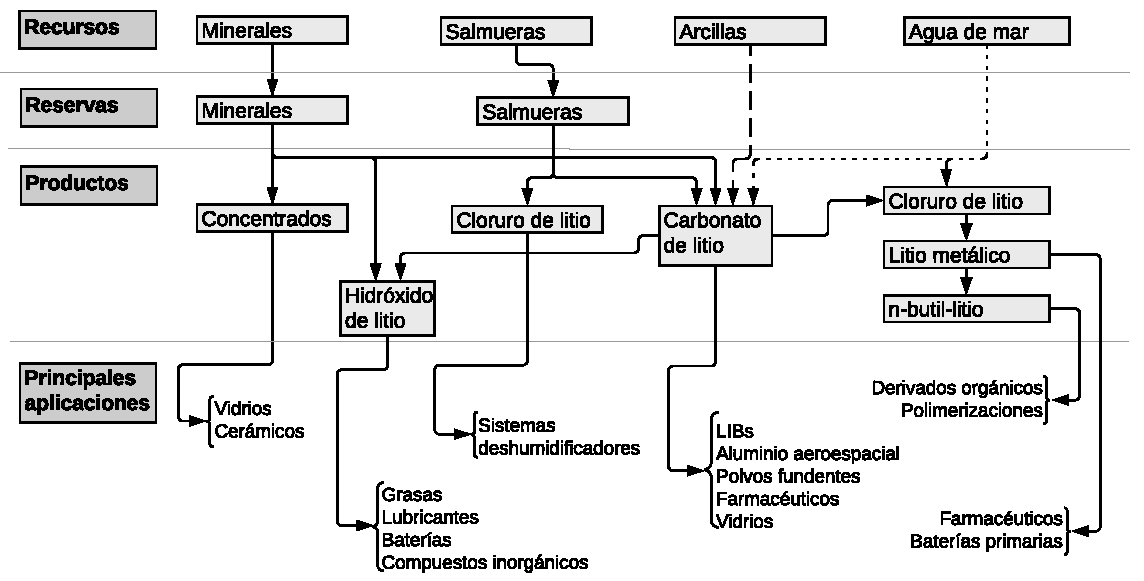
\includegraphics[width=\textwidth]{chap2/images/lithiumsoourcetoeum.pdf}
    \caption[Principales rutas del litio desde la fuente hasta su uso final.]{Principales rutas del litio desde la fuente hasta su uso final. Adaptado principalmente de \citet{SPEIRS2014}. La línea discontinua que desprende de arcillas es considerando el éxito de de proyectos como el de Bacadéhuachi-México y las líneas punteadas que desprenden de agua de mar son considerando la posible aplicación del presente proyecto.}
    \label{fig:esquemaSpiers}
\end{figure}
}

\subsubsection{Minerales en roca}\label{sec:pegma}
Los minerales de litio más relevantes se muestran en la Tabla \ref{tab:minerals} \citep{Anthony1995}. Estos minerales se presentan por lo general en forma de pegmatitas.\footnote{Rocas ígneas filolianas con intrusiones cristalinas} Las pegmatitas constituyen actualmente la mayor fuente de litio. Las minas más grandes de pegmatitas con litio están localizadas en Australia. La extracción del litio presente en esta matriz requiere inicialmente la destrucción del mineral por métodos mecánicos o químicos que demandan mucha energía y con frecuencia aumentan el costo de la extracción \citep{CHRISTMANN2015}.

\begin{table}[ht]
    \centering\footnotesize
    \begin{tabular}{@{}llrp{7cm}@{}}\toprule
        \textbf{Mineral} & \textbf{Fórmula empírica} & \textbf{Li (\%)} & \textbf{Detalles} \\\midrule
        Espomudena & \ce{LiAl(SiO3)2}      & 3.73 & Principal fuente mineral de litio.\\
        Lepidolita & \ce{KLi2AlSi4O10F(OH)}& 3.58 & Mineral de litio más abundante. Segunda fuente mineral más importante.\\
        Petalita   & \ce{LiAlSi4O10}       & 2.09 & Puede convertirse en Espomudena de alta calidad para su uso directo en cerámicos.\\
        Ambligonita& \ce{Li_{0.75}Na_{0.25}Al(PO4)F_{0.75}(OH)_{0.25}} & 3.44& Algunos yacimientos presentan hasta 10\% en masa de ion litio pero no es una fuente comercial importante por su baja abundancia.\\\bottomrule
    \end{tabular}
    \caption{Principales minerales (en roca) de litio.}
    \label{tab:minerals}
\end{table}

El mineral más importante de esta familia es la espomudena, cuyos concentrados pueden ser utilizados directamente como aditivo en vidrios y cerámicos, el segundo mercado final más importante del litio. Los concentrados son el resultado del beneficio de los minerales. Este proceso por lo general se realiza por medios mecánicos como flotación con líquidos densos y separación magnética \citep{TADESSE2019}. 

Para obtener compuestos de litio, el concentrado de mineral debe ser {tostado} a altas temperaturas en presencia de algún aditivo para formar compuestos lixiviables. Posteriormente el litio se concentra con resinas de intercambio iónico. Si se usa como aditivo, por ejemplo, ácido sulfúrico, se forman sales de sulfato que son lixiviables con agua caliente. Al elevar el pH del lixiviado acuoso, se eliminan por precipitación una parte importante de los cationes interferentes. La carbonatación de la disolución produce carbonato de litio, el compuesto más comercial de este elemento \citep{TRAN2015}.

\subsubsection{Salmueras}
Las salmueras de los salares componen actualmente los recursos más abundantes de litio. Los lagos salados con mayor cantidad de ion litio se encuentran en el triángulo del litio (ver Figura \ref{fig:recursos}), formado por Bolivia, Argentina y Chile. La concentración de ion litio en las salmueras de importancia comercial se encuentra entre 200 y 4000~mg~kg\mnn. La extracción del litio presente en estas matrices presenta la ventaja de que el elemento ya se encuentra en disolución y ya no son necesarias algunas de las etapas que consumen más energía cuando el litio se extrae a partir de minerales sólidos.

La obtención de compuestos de litio requiere inicialmente la eliminación de una porción importante del disolvente (agua), para concentrar el ion litio en el medio. Usualmente esto se hace por evaporación solar o por ósmosis inversa \citep{Swain2017}. El protocolo empleado en cada salmuera es diferente porque depende de las características del yacimiento. Si la salmuera contiene boro, este por lo general se retira con extracción por disolventes, porque el ácido bórico es un subproducto con valor comercial y porque el boro daña los sistemas de obtención de litio metálico a partir del cloruro de litio \citep{TRAN2015}. Los iones calcio y magnesio deben ser retirados por preci\-pi\-tación y posteriormente puede carbonatarse la disolución para precipitar carbonato de litio que posteriormente es purificado por recristalización o por filtración.

\subsubsection{Minerales en arcilla}\label{sec:arcillas}
Las  arcillas no son actualmente una fuente importante de litio, pero la situación promete cambiar próximamente con el avance de megaproyectos mineros ubicados principalmente en México y Estados Unidos. Las arcillas de litio más representativas se muestran en la Tabla \ref{tab:clays}. La más importante de este grupo es la hectorita. El proceso de extracción de litio a partir de estas matrices es similar al aplicado para obtener compuestos de litio a partir de rocas pegmatiticas.

\begin{table}[H]
    \centering\footnotesize
    \begin{tabular}{@{}llr@{}}\toprule
        \textbf{Mineral} & \textbf{Fórmula empírica} & \textbf{Li (\%)}\\\midrule
        Hectorita & \ce{Na_{0.3}(Mg,Li)_3Si_4O_{10}(OH)_2}  & 0.54 \\
        Jadarita & \ce{(Na,Ca)_{0,3(}Al,Mg)_2Si_4O_{10}(OH)_2.n(H_2O)}& -\\
        Polilitionita   & \ce{KLi_2AlSi_4O_10(F_{0.75}(OH)_{0.25})_2}       & -\\\bottomrule
    \end{tabular}
    \caption{Principales minerales (en arcillas) de litio.}
    \label{tab:clays}
\end{table}

El proceso de beneficio de las arcillas involucra un proceso de molienda fina y clasificación por tamaño de partícula usando un hidrociclón. Los aditivos añadidos en el tueste del concentrado son principalmente sulfato de sodio, sulfato de calcio (yeso) y carbonato de calcio (calcita). Se produce sulfato de litio que puede tratarse como se describió en la Sección \ref{sec:pegma} \citep{Bacanora2018}. Como subproducto de valor comercial se suele obtener sulfato de potasio.

\subsubsection{Agua de mar}
El ion litio se encuentra disuelto en el agua de mar a una concentración promedio de 0.18~mg~kg\mnn\ \citep{Evans2013}. Su concentración es diminuta, pero es el decimocuarto elemento más abundante en esta matriz. Como se ha mencionado en secciones anteriores, los océanos contienen el recurso de ion litio más grande conocido del planeta, y constituyen una fuente casi inagotable de este elemento \citep{Yang2018}; sin embargo, su extracción a escala industrial es inviable económicamente a causa de su baja concentración. Distintas metodologías son estudiadas actualmente para extraer ion litio a partir de esta matriz, pero se encuentran en etapa de investigación y desarrollo, por lo que se han incluido en la Sección \ref{sec:estadodelarte}.

\subsubsection{Reciclaje}

Actualmente, las cantidades de ion litio obtenidas por reciclaje no son importantes y puede que este panorama no cambie en un futuro próximo \citep{Olivetti2017}. El ion litio utilizado en cerámicos y vidrios no se puede recuperar \citep{CHRISTMANN2015}, y la minería urbana de \acp{LIB} por lo general se enfoca en la recuperación de cobalto o manganeso que tienen un mayor valor comercial. 

Algunas estimaciones establecen que para el 2050 el 25\% de la producción mundial de litio podría provenir de fuentes recicladas involucrando principalmente \ac{LIB}s. Este aumento del porcentaje sería en respuesta a la introducción al mercado masivo de baterías de ion litio de gran tamaño para \ac{EV}s, con el consecuente gran volumen de residuos que pueden representar dichas baterías hacia el final de su tiempo de vida útil (cerca de una década) \citep{STERBA2019416, Evans2013}. Predicciones sobre el crecimiento de la flota de vehículos eléctricos estiman que tan solo en los Estados Unidos podrían producirse hasta cuatro millones de toneladas de residuos de \ac{LIB}s en las próximas dos décadas \citep{RICHA2014}. 

Las \ac{LIB}s tienen entre 100 y 345~g de litio por cada kilowatt hora de capacidad. Esto representa cerca de 4~kg de litio en la batería de cada \ac{EV}. La dificultad principal que presenta el reciclaje del litio de estas fuentes recae en que la química de los cátodos empleados es muy variada (Tabla~\ref{tab:catodos}), y la minería urbana de este recurso se puede hacer menos eficiente dado que cada material requiere condiciones distintas de tiempo y composición, para la lixiviación eficiente de ion litio \citep{VENKATRAMAN2004}.% Políticas estrictas deberán establecerse para regular la recolección y clasificación de las baterías que han terminado su ciclo de vida.
\begin{table}[H]
    \centering\footnotesize
    \begin{tabular}{@{}p{3cm}lcp{5cm}@{}}\toprule
        \textbf{Nombre} &\textbf{Fórmula} &  \textbf{Energía específica}&\textbf{Detalles}\\
        &&(W~h~kg\mnn)\\\midrule
        Óxido de litio y cobalto (LCO) & \ce{LiCoO2} & 110-200 & Primer cátodo de uso industrial en \ac{LIB}s. Presenta desventajas de seguridad y ambientales, por riesgo de explosión y por el uso de cobalto, respectivamente.\\
        Óxido de litio, niquel, manganeso y cobalto & \ce{Li(Ni_{0.33}Mn_{0.33}Co_{0.33})O2} & 95-130 & Amplio uso en vehículos eléctricos.\\
        Espinela de litio y manganeso & \ce{LiMn2O4} & 110-120 & Bajo costo de producción. Amplio uso en vehículos híbridos eléctricos.\\
        Fosfato de litio y hierro & \ce{LiFePO4} & 95-140 & Es de los cátodos más seguros, con los menores costos de producción y con un bajo impacto negativo al medio ambiente\\\bottomrule
    \end{tabular}
    \caption[Principales materiales de los cátodos de LIBs.]{Principales materiales de los cátodos de \ac{LIB}s \citep{Chagnes2015}}
    \label{tab:catodos}
\end{table}

\subsection{Problemas socio-ambientales asociados}
El litio permite el funcionamiento de diversas tecnologías que prometen ayudar a disminuir el impacto ambiental negativo que acarrean muchas de las actividades humanas. A pesar de esto, su extracción y utilización no está libre de consecuencias para algunos de los ecosistemas y las poblaciones que rodean los yacimientos importantes.

El ejemplo más notorio lo presenta la extracción del ion litio presente en el Salar de Atacama en Chile, parte del triángulo del litio. La evaporación de grandes cantidades de agua de los salares para aumentar la concentración de ion litio resulta catastrófica para la fauna del lugar, porque el Desierto de Atacama es un lugar extremadamente seco y el acceso a las fuentes hídricas se encuentra injustamente restringido a su aprovechamiento comercial. Los reservorios subterráneos de estos salares son alimentados por fuentes acuáticas que también alimentan lagos que son muy importantes para las regiones circundantes. La minería de litio en esta región compite con los pobladores por el uso del agua y en los últimos  censos nacionales se ha evidenciado una caída importante en su población \citep{Romero2012, LIU202012}.

Por otro lado, el Salar de Uyuni, en Bolivia, es el segundo reservorio más grande conocido de ion litio (después de los océanos) con una excepcional estimación de 20 millones de toneladas de ion litio. Una dificultad importante que presenta la extracción de ion litio de este salar es que el ecosistema es muy delicado y el proyecto representaría una amenaza importante a la biodiversidad de la zona \citep{Hancock2018}. La protección de las especies endémicas de la región y de los pueblos indígenas que habitan la zona son un factor importante que afortunadamente han ralentizado el inicio de la explotación de este recurso.

Cuando la extracción de ion litio se hace a partir de rocas y arcillas, los procesos de calcinación y tueste tienen un gran impacto negativo al ambiente porque demandan altas cantidades de energía, liberan grandes volúmenes de emisiones atmosféricas, e involucran el uso de grandes cantidades de ácido \citep{Hancock2018}.

Los problemas sociales y ambientales de la extracción de ion litio a partir de agua de mar pueden ser significativamente menores que los asociados a los procesos de recobro a partir de salmueras y minerales rocosos o arcillosos. La cuasi-omnipresencia de los océanos permitiría ubicar los puntos de extracción en lugares donde el ecosistema sea robusto y no haya afectación a poblaciones humanas.

Respecto a los productos finales de litio, la fabricación de una batería con 1~kWh de capacidad requiere la inversión de cerca de 380~kWh de energía y el proceso puede liberar hasta 80~kg de \ce{CO2} \citep{Chagnes2015}. Al final de su ciclo de vida, estas baterías son consideradas residuos peligrosos que representan un peligro para el medio ambiente y para la salud de los humanos debido a sus altos contenidos de cobre, cobalto y níquel \citep{Kang2013}. El impacto negativo de estos residuos se mitigaría considerablemente con la implementación de políticas estrictas referentes al reciclaje de estos recursos.



\section{Estado del arte en el recobro de ion litio}\label{sec:estadodelarte}
Un gran número de metodologías se han propuesto para la separación selectiva de ion litio. En muchos casos los métodos han sido exitosamente aplicados a muestras reales, incluyendo agua de mar. En esta sección se resumen aspectos relevantes de estas técnicas. Las \acp{PIM} son tratadas independientemente en la Sección \ref{sec:pimint}.

La Tabla \ref{tab:ArtLitreports} resume algunos de los métodos recientes para la extracción de ion litio a partir de distintas matrices. De las técnicas incluidas, adsorción, intercambio iónico y electrólisis selectiva no comparten muchas características con el método propuesto en el presente trabajo. Por otro lado, la extracción con disolventes y con membranas líquidas soportadas contienen conceptos fácilmente adaptables a las \acp{PIM}. Este segundo grupo es analizado con más detalle en los siguientes apartados.

\clearpage
%\newgeometry{left=1cm, bottom=0.4cm, top=0.16cm}
\begin{landscape}%\thispagestyle{plain}
\centering
\begin{table}[H]
    \centering\footnotesize
    \begin{tabular}{@{}p{0.07cm}llcp{12cm}l@{}}\toprule
        &\textbf{Material o Reactivo} &\textbf{Matriz}&\textbf{Eficiencia}&\textbf{Detalles}&\textbf{Referencia} \\&&&\textbf{(\%)}\\\midrule
        \multicolumn{3}{@{}l}{\textit{Extracción con disolventes}}\\
        &LIX-54/Cyanex 923&Sintética&98&\textbf{Rel. mol.}: 2:1 (LIX-54:Cyanex 923). \textbf{Dil}: ShellSol D70 (Parafinas y naftenos C11-C14).\newline Efecto sinérgico entre los extractantes. & \citet{Pranolo2015}\\
        &LIX-54/TOPO & Sintética &- & \textbf{Dil}: Queroseno.\newline Efecto sinérgico entre los extractantes.  &\citet{Kunugita1989}\\
        &TTA/TOPO & Agua de mar & 65& \textbf{Dil}: Queroseno.\newline Efecto sinérgico entre los extractantes. El magnesio fue precipitado con \ce{NH4OH}. & \citet{Harvianto2016}\\
        &\ce{[N4444][EHEHP]}&Sintética&95& \textbf{Dil}: Dicloroetano.&\citet{Shi2020}\\
        &TBP&Sintética&65& \textbf{Dil}: Succinato de dietilo. \textbf{Cox}:\ce{FeCl3}. &\citet{Zhou2020}\\
        
        \multicolumn{3}{@{}l}{\textit{Membranas líquidas Soportadas}}\\
        &LIX-54/TOPO& Sintética&90&\textbf{Rel. mol.}: 3:1 (LIX-54:TOPO). \textbf{Dil}: Queroseno. \textbf{Rec}: \ce{H2SO4} (1~mol~L\mnn)&\citet{Ma2000}\\
        &D2EHPA/TBP & Sintética&82&\textbf{Dil}: Queroseno. \textbf{Rec}: \ce{HCl}  &\citet{sharma2016}\\
        &\ce{[C4mim][NTf2]}/TPB& Sintética &70 & \textbf{Pol}:  poli(1,1-difluoroetileno). \textbf{Rec}: \ce{Na2CO3 + NaHCO3} (2~mol~L\mnn)&\cite{ZANTE2019}\\
        
        \multicolumn{3}{@{}l}{\textit{Adsorción e intercambio iónico}}\\
        &\ce{H_{1.6}Mn_{1.6}O4}&Agua de mar &85&\textbf{Cap}: 40~mg~g\mnn&\citet{Chitrakar2001}\\
        &\ce{H_{1.33}[Ti_{x}Mn_{1-x}]_{1.67}O4}&Agua de mar&-&\textbf{Cap}: 22~mg~g\mnn &\citet{RYU2019}\\
      %  &HMO/Celulosa& & &\citet{Tang2020}\\
        
        \multicolumn{3}{@{}l}{\textit{Métodos electroquímicos}}\\
        &\ce{[PP13][NTf2]}&Agua de mar & -&Electrólisis de membrana líquida soportada con líquido iónico como extractante.&\citet{Hoshino2014}\\
        &LISICON& Agua de mar & - & Electrólisis de membrana selectiva a litio (LISICON)\newline Obtención directa de litio metálico. La celda funciona con energía solar. &\citet{Yang2018}\\
        &CEM/BLM/CEM& Sintética & 49 &\textbf{Rec}: HCl (0.03~mol~L\mnn)\newline Electrólisis de membrana líquida (TBP) intercalada entre dos CEMs &\citet{ZHAO2020}\\
        
        
        
        \multicolumn{3}{@{}l}{\textit{Membranas poliméricas de inclusión}}\\
        &TTA/TOPO & Sintética & &\textbf{Rel. mol.}:  2:1 (TTA:TOPO). \textbf{Rec}: HCl (0.1~mol~L\mnn)\newline La membrana pierde el 64\% de su eficiencia tras el cuarto ciclo de reuso.   &\citet{Cai2019}\\
        &\textbf{LIX-54/Cyanex 923} & \textbf{Agua de mar} &  &\textbf{Rel. mol.}: 2.15:1 (LIX-54:Cyanex 923)  \textbf{Rec}: HCl (0.1~mol~kg\mnn) \newline La membrana pierde menos del 40\% de su eficiencia tras el décimo ciclo de reuso.&\textbf{Este trabajo}\\\bottomrule   
        
       \multicolumn{6}{@{}p{23.5cm}@{}}{\scriptsize 
        \textbf{LIX-54}: 1-fenildecanona-1,3-diona. \textbf{Cyanex 923}: Mezcla de óxidos de trialquil fosfinas. \textbf{TOPO}: Óxido de trioctilfosfina. \textbf{TTA}: Teonil trifluoroacetona.          \textbf{\ce{[N_{4444}][EHEHP]}}: 2-etilhexilhidrogeno-2-etilhexilfosfonato de tetrabutilamonio.
        \textbf{TBP}: Tributilfosfato. \textbf{D2EHPA}: Ácido Di-(2-etillhexil)fosfórico.       \textbf{\ce{[C4mim][NTf2]}}: bis(trifluorometilsulfonilimida) de 1-butil-3-metilimidazolio. \textbf{\ce{[PP13][NTf2]}}:  bis(trifluorometilsulfonilimida) de N-metil-N-propilpiperidinio. %\textbf{HMO}: Óxido metálico con hidrógeno.  
        \textbf{LISICON}: Membrana superiónica conductiva de litio. \textbf{CEM}: Membrana de intercambio catiónico.\newline \textbf{BLM}: Membrana líquida \textit{de bulto}.
        \newline\textbf{Rel. mol.}: Relación molar de extractantes.
        \textbf{Dil}: Diluente de los extractantes. 
        \textbf{Cox}: Agente de coextracción.
        \textbf{Pol}: Polímero soporte. 
        \textbf{Rec}: Fase receptora o de recuperación. 
        \textbf{Cap}: Capacidad específica de adsorción de litio}
    \end{tabular}
    \caption{Métodos del estado del arte en extracción de litio.}
    \label{tab:ArtLitreports}
\end{table}
\end{landscape}

\subsection{Extracción con disolventes}\label{sec:extr.disolv}\index{Extracción!con disolventes}
La extracción con disolventes (o extracción líquido-líquido) se fundamenta en el reparto preferencial de un soluto entre dos fases líquidas inmiscibles que se encuentran en contacto. El reparto preferencial de dicho soluto en una fase o la otra depende en parte de la solubilidad que este presenta en cada uno de los medios. Con regularidad se emplean disolventes orgánicos para extraer cationes metálicos que se encuentran en medio acuoso. La solubilidad de estos solutos es bastante baja en el medio orgánico debido a la naturaleza de los cationes y de los disolventes orgánicos. Debido a esto, usualmente se incorporan en la fase orgánica extractantes orgánicos que forman compuestos estables neutros con los cationes y favorecen su reparto. Esto se conoce como extracción facilitada. En un segundo paso, el proceso es revertido usando una nueva disolución acuosa a partir de la cual, en pasos posteriores, pueden obtenerse compuestos de alta pureza del elemento en cuestión \citep{NARBUTT2020}. La primera disolución acuosa que contiene originalmente la especie de interés es denominada fase donadora o de alimentación, mientras la segunda se llama fase receptora o de recuperación. Las etapas de la separación se conocen como extracción y recuperación, respectivamente. Las condiciones de la extracción pueden ser finamente ajustadas a tal punto que incluso se hace posible la separación isotópica de distintos elementos. \citet{LIU2018c} reportaron el uso de éteres corona para la separación isotópica de \ce{^6Li}. Este isótopo es de gran importancia para la producción de tritio (\ce{^3H}) que se emplea en algunos reactores nucleares.

Los extractantes \index{Extractantes} que facilitan la extracción pueden dividirse en tres grupos principales, acorde al mecanismo de interacción con la especie que se extrae:
\begin{itemize}
    \item Extractantes ácidos (intercambiadores catiónicos)
    \item Extractantes alcalinos (intercambiadores aniónicos)
    \item Extractantes neutros (agentes solvatantes)
\end{itemize}

Los extractantes alcalinos son útiles en la extracción de especies con carga negativa. El ion litio no forma compuestos aniónicos bajo las condiciones del presente estudio, por lo que estos extractantes no son de interés en este trabajo.

En los extractantes ácidos (representados como \ce{HL}), la especie de interés (\ce{M^n+}) desplaza protones ácidos que son donados al medio acuoso para formar un complejo neutro (\ce{ML_n}), que por lo general es soluble en la fase orgánica:
\begin{equation}
    \ce{M^{n+} + n\overline{HL} <=> \overline{ML_n} + nH^+}
\end{equation}
donde la barra horizontal superior denota que la especie se encuentra en la fase no acuosa. 

Los agentes quelantes (\ce{B}), involucran la complejación de especies neutras (\ce{MX_n}) para formar un complejo también neutro (\ce{MX_nB_b}) que es altamente soluble en la fase orgánica:
\begin{equation}
    \ce{M^{n+} + nX^{-} + b\overline{B} <=> \overline{MX_nB_b}}
\end{equation}
En varios casos, los extractantes ácidos pueden reaccionar con el catión de interés como intercambiador catiónico y como agente solvatante, de manera simultánea \citep{Swain2016}:
\begin{equation}
    \ce{M^{n+} + (n + m)\overline{HL} <=> \overline{ML_n(HL)_m} + nH^+}
\end{equation}

La extracción de ion litio utilizando únicamente extractantes neutros es difícil, por lo que usualmente se requiere la adición de un anión anfifilico\footnote{Afín a ambas fases: acuosa y orgánica.} que permita la posterior solvatación del par iónico formado, por parte de la molécula extractante. \citet{Zhou2020} reportaron la utilidad del cloruro de hierro(III), que en medio acuoso con cloruros forma el complejo tetracloroferrato(III), para facilitar la solvatación de ion litio, usando un extractante orgánico neutro (TBP).

Un enfoque común para la extracción de cationes metálicos consiste en la combinación de un extractante ácido con uno neutro. La combinación de estos extractantes puede dar lugar a procesos que son más eficientes que la suma de las eficiencias de los procesos realizados con dichos extractantes de manera individual.  Esto se conoce como efecto sinérgico y ha sido ampliamente aplicado a la extracción de ion litio \citep{Pranolo2015, Kunugita1989, Harvianto2016}. La dificultad que presentan los extractantes ácidos para extraer por sí mismos al ion litio recae en que su número de coordinación es de cuatro \citep{Kinugasa1994}, y el extractante no satisface las necesidades de coordinación del ion litio. Los espacios remanentes son ocupados con moléculas de agua, formando una esfera de hidratación que hace el complejo incompatible con la fase orgánica altamente hidrofóbica. Estos espacios disponibles en el compuesto neutro formado por la base conjugada del extractante ácido y el ion litio, pueden ser ocupados por un agente quelante lipofílico que permita la incorporación del compuesto final a la fase orgánica \citep{NARBUTT2020}.

En algunos casos, la extracción con disolventes es aplicada para la extracción de los cationes calcio y magnesio que impiden la precipitación de compuestos de litio de alta pureza \citep{Shi2020b}. Este enfoque es ventajoso desde un punto de vista práctico, dado que los cationes divalentes son solvatados con mayor fuerza que los cationes monovalentes y, por lo tanto, su proceso de extracción es más rápido y sencillo.

\subsection{Membranas líquidas soportadas}\index{Extracción!con membranas líquidas soportadas}
Una membrana es una barrera física semipermeable que separa dos medios. Las membranas líquidas pueden ser soportadas (membrana líquida soportada (SLM)\acused{SLM}) o no soportadas (como las membranas líquidas de bulto (BLM) \acused{BLM}). Las \ac{SLM}s consisten en un soporte polimérico poroso impregnado con un disolvente orgánico que incorpora las moléculas extractantes. El uso de estas membranas representa una evolución de la extracción por disolventes y resuelve bastantes problemas relacionados con dicha metodología. Las etapas de extracción y de recuperación se llevan a cabo simultáneamente en un proceso que involucra cantidades de disolventes y de extractantes mucho menores a los usados en la extracción con disolventes. Esto representa ventajas operacionales y ambientales muy grandes. Su versatilidad las hace muy atractivas para distintas aplicaciones. Numerosas separaciones de iones metálicos han sido logradas usando este tipo de membranas \citep{deGyves1999}.

La separación de iones metálicos por medio de \ac{SLM}s puede lograrse con la adaptación de sistemas de extractantes y disolventes previamente reportados en la extracción con disolventes para el ion de interés. \citet{Ma2000} usaron en una \ac{SLM} los mismos extractantes diluidos en el mismo disolvente del sistema de extracción por disolventes reportado por \citet{Kunugita1989}. Los efectos sinérgicos entre extractantes ácidos y neutros reportados en la extracción de ion litio por disolventes, también son posibles (y muchas veces, necesarios) en la extracción usando \ac{SLM}s.

El principal inconveniente que presentan las \ac{SLM}s reside en la poca estabilidad que presentan a causa de fenómenos como emulsión de la fase orgánica en las fases acuosas, o volatilización del disolvente que diluye los extractantes. Estos inconvenientes pueden ser subsanados con el uso de líquidos iónicos como extractantes \citep{ZANTE2019}, o modificando la estrategia de la separación, usando otro tipo de membranas más estables, como las membranas poliméricas de inclusión.

La mayoría de los parámetros de desempeño relacionados con las \ac{SLM}s son comunes con los de las \acp{PIM} y por lo tanto, son tratados en la siguiente sección.
%\subsection{Métodos electroquímicos}
%\citep{Yang2018} LESS: 7828220525
%\citep{ZHAO2019}

%\subsection{Adsorción selectiva}
%Recovery of lithium in seawater using a titanium intercalated lithium manganese oxide composite
%Author links open overlay panelTaegongRyu
%10.1016/j.hydromet.2018.12.012


%\subsection{Adsorción selectiva e intercambio iónico}
%Recurrentemente se han estudiado materiales sólidos con alta selectividad hacia el litio para la separación selectiva de este elemento a partir de salmueras y de agua de mar \cite{ARROYO2019}. Los materiales más utilizados son óxidos metálicos (principalmente de manganeso) que capturan selectivamente iones litio en su estructura cristalina o resinas de intercambio catiónico en las que el litio reemplaza posiciones ocupadas por iones hidronio. En muchos casos los adsorbentes y las resinas empleadas se encuentran disponibles comercialmente.

%El protocolo involucra el contacto íntimo entre la disolución con litio (disolución de alimentación) y el adsorbente o la resina de intercambio iónico. Cuando el material sólido se ha cargado con litio al máximo de su capacidad se lava y se repite el proceso de contacto íntimo usando esta vez una disolución de recuperación generalmente compuesta de ácido clorhídrico diluido. En la segunda etapa, el litio es retirado del material sólido con lo que éste es regenerado y puede usarse nuevamente. Si se reutiliza la disolución de recuperación o si el volumen empleado es menor al de la disolución de alimentación puede concentrarse el litio y esto facilita la posterior obtención de compuestos sólidos.

%Algunas variaciones involucran los materiales sólidos para retirar del medio a todos los cationes exceptuando al litio que queda en disolución. \citet{Nishihama2011} reportaron el uso secuencial de resinas de intercambio iónico para eliminar los cationes alcalinos y alcalinotérreos que podrían interferir en la precipitación de litio a partir de un concentrado de agua de mar. Luego de eliminar los interferentes el litio pudo ser precipitado usando carbonato de amonio para obtener carbonato de litio con una pureza mayor a 99.9\%.

%\subsection{No se como llamar lo de acá D:0\}}
%Innovative lithium recovery technique from seawater by using world-first dialysis with a lithium ionic superconductor
%https://doi.org/10.1016/j.desal.2014.12.018





\section{Membranas poliméricas de inclusión}\label{sec:pimint}\index{PIM}
Las membranas poliméricas de inclusión (PIM) son un tipo de membranas líquidas que incorporan extractantes en la red polimérica de un termoplástico no poroso. Las \ac{PIM}s tienen las ventajas que presentan las \ac{SLM}s (unificación de los pasos de extracción y recuperación, bajo consumo de extractantes y de disolventes), y superan el principal inconveniente de este tipo de membranas relacionado con su pobre estabilidad \citep{Nghiem2006}. A diferencia de las SLM, en una PIM los extractantes no se encuentran disueltos en un disolvente que está impregnado en los canales de una membrana porosa, sino que se encuentran absorbidos en la red polimérica por fuerzas capilares y de unión no covalente. Dado que los extractantes no se encuentran en contacto tan directo con las disoluciones acuosas, son más resistentes frente a la lixiviación. 

Las \ac{PIM}s se encuentran en aplicaciones que van más allá de la separación selectiva de especies en disolución. Han sido utilizadas en distintas técnicas analíticas de cuantificación de especies (por métodos electroquímicos y espectrofotométricos), y de pretratamiento de muestras (preconcentración de especies y muestreo pasivo) \citep{ALMEIDA2017}. La separación selectiva de especies en disolución utilizando PIMs puede ser con fines extractivos, o para disminuir la peligrosidad de residuos mineros, industriales, y nucleares \citep{Kolev2019}.

El polímero base generalmente es de triacetato de celulosa (CTA) \acused{CTA} o de poli(cloruro de vinilo) (PVC) \acused{PVC}. El polímero se encarga de dar forma a la membrana y de proveerle resistencia mecánica. En la mayoría de los casos, se hace necesaria la adición de un plastificante que provee flexibilidad al polímero por medio de la disminución en las interacciones entre las cadenas poliméricas. Sin embargo, a veces la adición de un plastificante no es necesaria, pues las moléculas del extractante pueden cumplir también esa función. 

%\subsection{Extractantes}
%Los extractantes son la parte más importante en la \ac{PIM}. Las interacciones de estas moléculas con las especies en disolución dependen fuertemente de la naturaleza de la especie en cuestión por lo que éstos son los encargados de proveer la selectividad del proceso. Los extractantes 
    
%En la extracción de litio usando \ac{SLM}s o \ac{SSX} es común la combinación de un extractante ácido con un agente quelante. La combinación de extractantes de esta naturaleza presenta efectos sinérgicos que permiten la separación de litio que es muy difícil o imposible usando los mismos extractantes individualmente.

\subsection{Parámetros de desempeño}\label{sec:performanceparameters}
Una PIM puede caracterizarse por medio de la mayoría de las técnicas ampliamente esparcidas en la ciencia de materiales (e.g.\ microscopías electrónicas, análisis térmicos, métodos electroquímicos, y espectrofotométricos). Cuando el propósito de la \ac{PIM} es transportar un elemento con el fin de lograr su recobro, es particularmente importante conocer la eficiencia con la que se lleva a cabo el proceso y el coeficiente de permeabilidad que está directamente relacionado con el flujo de la especie en cuestión a través de la membrana. Se espera que dicho recobro sea selectivo y la magnitud que permite juzgar la selectividad de un sistema es el factor de separación. Adicionalmente, desde un punto de vista práctico, una membrana robusta que pueda usarse varias veces es más viable que una membrana que solo funciona una vez. Los cambios en las propiedades de transporte de una membrana en el tiempo como consecuencia de alteraciones estructurales fisicoquímicas se conoce como su envejecimiento físico \citep{Koros}.

La eficiencia ($E$) en el proceso de transporte estudiado se relaciona con la concentración de ion litio que ha sido alcanzada en la fase de recuperación a un determinado tiempo $t$, respecto a la concentración inicialmente presente en la fase de alimentación. Usualmente se reporta en términos de porcentaje. Los datos del transporte pueden presentarse como fracción remanente en la disolución de alimentación ($\Phi_{ali}$), y fracción transportada a la disolución de recuperación ($\Phi_{rec}$), en función del tiempo. En este caso, la eficiencia se hace equivalente a la fracción transportada a la disolución de recuperación, en porcentaje.
\begin{equation}\label{eq:efi}
    E(t)=\frac{[\ce{Li^+}]_{rec}(t)}{[\ce{Li^+}]_{ali}^0}\times100\% = \Phi_{rec}(t)\times100\%
\end{equation}

El coeficiente de permeabilidad ($P$) \index{Coeficiente de permeabilidad} se define como el flujo transportado a través de una membrana por unidad de fuerza motriz (gradiente de potencial químico en nuestro caso), por unidad de grosor de la membrana \citep{Koros}. En membranas líquidas se asume que las reacciones de formación/disociación de aductos en las interfases de la membrana son más rápidas que el proceso de difusión de la especie a través de la membrana. En ese caso, la ley de difusión de Fick en estado estacionario puede escribirse \citep{Ma2000}:
\begin{equation}\label{eq:fick}
    P=-\frac{d[\ce{Li^+}]_{ali}(t)}{dt}\times\frac{V}{a}\times\frac{1}{[\ce{Li^+}]_{ali}(t)}
\end{equation}
Donde $V$ es el volumen inicial de la disolución de alimentación y $a$ es el área expuesta de la membrana. La Ecuación diferencial \ref{eq:fick} puede resolverse por separación de términos e integración considerando que $[\ce{Li^+}]_{ali}(t=0)=[\ce{Li^+}]_{ali}^0$:
\begin{equation}\label{eq:coefPerm}
    \ln{\Bigg(\frac{[\ce{Li^+}]_{ali}(t)}{[\ce{Li^+}]_{ali}^0}\Bigg)}=\ln(\Phi_{ali}(t))=-\frac{P~a}{V}t
\end{equation}
En ese orden de ideas, el logaritmo natural de la fracción remanente de ion litio en la fase de alimentación debería ser una relación lineal negativa con el tiempo. A partir de la pendiente de dicha relación puede obtenerse el coeficiente de permeabilidad.

El factor de separación \index{Factor de separación} de ion litio frente a otro catión \ce{M^n+} ($Sf_{\ce{Li+}/\ce{M^n+}}$), se define como la relación de sus concentraciones en la disolución de recuperación respecto al valor inicial de esta relación en la fase de alimentación \citep{Chen2018}. Otras definiciones usan en el denominador la relación de las concentraciones en la disolución de alimentación al mismo tiempo $t$ \citep{Koros, sharma2016}. Estas definiciones son más apropiadas para sistemas de separación en sistemas continuos, y por lo tanto pueden conducir a conclusiones erróneas en sistemas como el trabajado en el presente proyecto. El factor de separación debe ser igual a uno al comienzo del experimento, indicando que no ha ocurrido separación de especies. Factores de separación más grandes implican mejor selectividad por la especie de interés. Un factor de separación menor a uno indica que la especie que no es de interés es transportada con preferencia a través de la membrana, es decir, que el sistema no es selectivo frente a dicha especie.
\begin{equation}
    Sf_{\ce{Li^+}/\ce{M^n+}}(t)=\frac{[\ce{Li^+}]_{rec}(t)/[\ce{M^n+}]_{rec}(t)}{[\ce{Li^+}]_{ali}^0/[\ce{M^n+}]_{ali}^0}
\end{equation}

Cuando el envejecimiento físico de la membrana es consecuencia de su utilización, éste puede determinarse de manera inversa como la estabilidad que presentan sus propiedades de transporte tras un número determinado de ciclos de uso.  La estabilidad de las PIMs es una de sus principales ventajas frente a otros sistemas de separación, y es quizás el parámetro clave que puede impulsar su aplicación en el mundo real. 

Finalmente, una manera práctica de evaluar el desempeño de un sistema frente a una sustancia es a través de su perfil de transporte, \index{Perfiles de transporte} que muestra gráficamente las fracciones o concentraciones de una o más especies, en las fases de alimentación y de recuperación, en función del tiempo. Los perfiles de transporte dan cuenta de la eficiencia de la extracción y la velocidad a la que ocurre el proceso. Si se incluye más de una especie en el perfil de transporte, esta herramienta también otorga información de la selectividad con la que se lleva a cabo el proceso.


\subsection{Mecanismo de extracción de ion litio con el sistema propuesto}
Para que una especie logre ser transportada a través de una \ac{PIM}, primero debe formarse el complejo de la especie de interés con los extractantes de la membrana en la interfase de la membrana con la disolución de alimentación, y dicho complejo debe difundir hasta la interfase de la membrana con la disolución de recuperación. Finalmente, el compuesto formado debe disociarse para liberar la especie en cuestión hacia la disolución de recuperación. Las reacciones que presenta el ion litio con los extractantes escogidos se tratan en este apartado.

Los procesos de transporte que involucran el transporte activo de sustancias facilitado por extractantes a través de PIMs, pueden utilizar como fuerza motriz el contratransporte de un catión, o de un anión, que se encuentra a altas concentraciones en la disolución de recuperación. También puede aprovecharse el cotransporte de un anión, o de un catión, que se encuentra a altas concentraciones en la disolución de alimentación \citep{Nghiem2006}. En el caso del transporte de ion litio, el proceso es impulsado por el contratransporte de iones hidronio que son tomados de la disolución de recuperación, y son liberados en la disolución de alimentación cada vez que se toma un ion litio de este medio.

Como se mencionó en la Sección \ref{sec:extr.disolv}, el número de coordinación del ion litio es de cuatro, y en medio acuoso la especie que predomina es el ion tetrahidratado \citep{Kinugasa1994}. Las aguas de hidratación del ion dificultan su paso a través de la membrana de \ac{CTA}, que es de naturaleza hidrofóbica \citep{Nghiem2006}. Las reacciones de formación y disociación de aductos que tienen lugar en las interfaces de la \ac{PIM} con las disoluciones de alimentación y de recuperación son prácticamente las mismas que se presentan en los sistemas análogos de extracción sinérgica con disolventes (SSX)\acused{SSX}, reportado por \citet{Pranolo2015}, y con \ac{SLM}, reportado por \citet{Ma2000}. Debe considerarse que a diferencia de las extracciones con disolventes, la cantidad de extractante disponible para reaccionar en una PIM puede ser limitada respecto a la cantidad de iones objetivo que deben ser transportados. Esto puede justificar que la selectividad de estos sistemas no necesariamente tiene que ser igual a la observada en los sistemas análogos de extracción por disolventes \citep{Nghiem2006}. 

Las reacciones que pueden estar ocurriendo en la interfase membrana/disolución-de-alimentación incluirían, en una primera etapa, la formación de un complejo del tautómero enólico del LIX-54-100 con el ion litio:

\begin{equation}\label{eq:li1}
    \scriptsize\schemestart
    \chemleft\{\chemfig{O=[:180]
        (-[:120](-[:60](=[:0]O)(-[:120,,,1]R_1)))
        (-[:-120]R_2)}\chemright.
     \arrow{<->} 
    \chemleft. \chemfig{O=[:180]
        (-[:120](=[:60]((-[:0]O-[:-30]H))(-[:120,,,1]R_1)))
        (-[:-120]R_2)}\chemright\}
    \,+\,
    \chemleft[\chemfig{\color{black}{Li^+}
    (-[:45,1.4,,,<-]OH_2)
    (-[:135,1.4,,,<-]H_2O)
    (-[:-45,1.4,,,<-]OH_2)
    (-[:-135,1.4,,,<-]H_2O)}\chemright]
    \arrow{<=>[-\ce{2H2O}][+\ce{2H2O}]}
    \chemleft[\chemfig{\color{black}{Li}
    (-[:45,1.2,,,<-]OH_2)
    (-[:135,1.2,,,]O
        -[:180](-[:120,,,1]R_1)(=[:-120]))
    (-[:-45,1.2,,,<-]OH_2)
    (-[:-135,1.2,,,<-]O
        =[:180](-[:120])(-[:-120]R_2))}\chemright] 
    \arrow{0}[,0]
    \,+\, \ce{H+}
    \schemestop
    %\bigskip
\end{equation}\\[0.01ex]
donde \ce{R_1} y \ce{R_2} pueden ser sustituyentes fenil y heptil.

En una segunda etapa, las dos moléculas de aguas de hidratación remanentes en la esfera de solvatación del ion litio son desplazadas de este lugar por el extractante solvatante Cyanex~923, con lo que el aducto resultante es altamente hidrofóbico y puede ser transportado a través de la membrana.

\begin{equation}\label{eq:li2}
    \scriptsize\schemestart
    \chemleft[ \chemfig{O(-[:45,,,,->])(=[:180]
        (-[:120](=[:60]((-[:0]O-[:-45,1.1]Li(-[:-45,1.2,,,<-]OH_2)(-[:45,1.2,,,<-]OH_2)))
        (-[:120,,,1]R_1)))
        (-[:-120]R_2))}\chemright]
    \,+\,
    \chemfig{P(=[:90]O)(-[:-45,1.3]R_3')(-[:-75,1.3]R_2')(-[:-115,1.3]R_1')}
    \arrow{<=>[-\ce{2H2O}][+\ce{2H2O}]}
    \chemleft[ \chemfig{O(-[:45,,,,->])(=[:180]
        (-[:120](=[:60]((-[:0]O-[:-45,1.1]Li(-[:30,1.3,,,<-]O(=[:-90, 1.3]P
            (-[:-45,1.3]R_3')(-[:-75,1.3]R_2')(-[:-115,1.3]R_1')))-[:-30,1,,,<-]))
        (-[:120,,,1]R_1)))
        (-[:-120]R_2))}\chemright]
    \schemestop
    \bigskip
\end{equation}
donde \ce{R_1}', \ce{R_2}', y \ce{R_3}' son cadenas alquílicas con seis u ocho átomos de carbono.

Las Reacciones \ref{eq:li1} y \ref{eq:li2} ocurren en la dirección planteada en la interfase con la disolución de alimentación, y en la dirección contraria en la interfase con la disolución de recuperación. El resultado neto es el transporte de ion litio hacia la disolución de recuperación con el  consecuente transporte de iones hidronio hacia la disolución de alimentación.



%\section{Técnicas de cuantificación empleadas}
%\subsection{Espectrometría de Absorción Atómica por Llama}
%\subsection{Espectrometría de Emisión Atómica por Llama}
%\subsection{Curva de calibración por patron externo}
%\subsection{Curva de calibración multivariada}
%\subsection{Adición estándar de un solo punto}

\section{Diseño de experimentos y optimización}\label{sec:DoE}\index{Diseño de experimentos}
En las ciencias exactas es común el estudio de sistemas en los que se busca relacionar un fenómeno con sus posibles causas. En algunos casos dicho conocimiento permite controlar o predecir propiedades de interés del sistema (i.e.\ variables respuesta), tomando como base las condiciones que se cree que gobiernan al fenómeno en cuestión (i.e.\ variables explicatorias). Las variables explicatorias pueden estar compuestas por factores difíciles o imposibles de controlar (e.g.\ condiciones metereo\-lógicas), o bien, por parámetros que pueden ser ajustados al criterio del experimentador.

Tradicionalmente, esta clase de estudios se han hecho por un enfoque de una variable a la vez en la que se mantienen constantes la mayor cantidad posible de factores, a excepción de una variable que es modificada para buscar su relación con la variable respuesta de interés. Cuando se ha establecido esa relación, se escoge un valor conveniente que es fijado para la variable explicatoria recién estudiada, y el proceso se repite consecutivamente con otra variable hasta que todas han sido estudiadas. Esta metodología ha permitido aportes muy significativos en distintos campos y aún hoy por hoy es la opción predilecta por muchas personas que trabajan en campos muy importantes de la ciencia. Sin embargo, el enfoque de una variable a la vez presenta algunas limitaciones como el requerir un gran número de corridas experimentales y no evaluar las posibles interacciones entre variables explicatorias. Una consecuencia común de estas falencias metodológicas recae en que las condiciones encontradas como {óptimas} dependen en gran medida del orden en que son estudiadas las variables. En muchos casos esto implica que no se determine el punto óptimo real de un sistema.

Los diseños de experimentos y los algoritmos de optimización comprenden un conjunto de herramientas estadísticas y matemáticas que facilitan la planeación eficiente y el análisis objetivo de conjuntos experimentales. El propósito de estas herramientas es obtener la mayor cantidad posible de información de un sistema, o de llegar a su configuración más apropiada para un fin determinado (i.e.\ el punto óptimo), en un reducido número de experimentos \citep{Box2005}. 

Los conceptos de esta rama de la ciencia pueden ser aplicados para encontrar las mejores condiciones para el transporte de ion litio usando PIMs, considerando por ejemplo, el efecto de la formulación de la membrana en la eficiencia y la selectividad de los sistemas propuestos. En el desarro\-llo de esta tesis se han utilizado en particular los diseños experimentales fraccionados de dos niveles y el algoritmo de optimización simplex modificado. Las características más importantes de estos conceptos se exponen en las siguientes subsecciones.

\subsection{Diseño factorial fraccionado}\label{sec:FrF2introd}\index{Diseño de experimentos!factorial fraccionado}
En los diseños experimentales factoriales se estudia un número de variables $k$ en un número de niveles $n$ considerando todas las combinaciones posibles. El número de experimentos que deben realizarse es de $n^k$. Este valor crece considerablemente cuando se incluyen más niveles o variables. Aunque puede obtenerse información muy detallada del sistema, llevar a cabo un número tan grande de experimentos no es conveniente en la mayoría de los casos desde un punto de vista práctico. En el caso más simple y más famoso, los diseños experimentales factoriales son reducidos a solo $n=2$ niveles, pero el número de experimentos que deben realizarse en el estudio de $k$ variables sigue creciendo de manera exponencial a medida que se desea considerar más factores. La realización de $2^k$ experimentos permite, en principio, conocer el efecto de todas las variables en el sistema, incluyendo todas las interacciones que pueden presentar estas entre sí.

Con regularidad, la evaluación de las interacciones de alto grado (i.e.\ entre muchas variables) puede resultar de poca relevancia práctica, dado que la mayoría de las veces el efecto de dicha interacción no puede distinguirse del mero error aleatorio del proceso. En otras palabras, no es estadísticamente significativo. Esta consideración permite la realización de un número de experimentos mucho menor a expensas de la imposibilidad de determinar interacciones que se consideran poco importantes. Este es el principio de los diseños factoriales fraccionados en los que solo una fracción de la matriz de diseño es evaluada. La fracción debe escogerse cuidadosamente, de manera tal que la porción que se descarta no impida la evaluación de los efectos que se desea evaluar. Convenientemente, los algoritmos que permiten la elección de la {mejor fracción} se encuentran implementados en muchos programas y paquetes estadísticos \citep{FrF2}, por lo que esta decisión no es un problema para el experimentador en estos tiempos modernos.

Por ejemplo, en un diseño experimental factorial en el que se desea estudiar siete variables a dos niveles, el número de experimentos que debe correrse es de $2^7=128$. Sí se acepta que la interacción entre más de cuatro variables no es relevante, el mismo número de variables puede ser evaluado en $2^{7-1}=64$ experimentos. La reducción en el tiempo que debe invertirse es drástica. De manera análoga, si se ignoran las interacciones entre tres y en el caso más extremo, las interacciones entre parejas de variables, el número de experimentos a realizarse decrece a $2^{7-3}=16$ y $2^{7-4}=8$, respectivamente. 

Debe considerarse que los efectos de las interacciones entre variables no {desaparecen} cuando se decide que no es importante su determinación. Estos efectos se solapan con aquellos de inter\-accio\-nes de menor grado y con efectos de variables individuales. Cuando esto ocurre se dice que los efectos están {confundidos}. El hecho de que algunos efectos de variables puedan estar confundidos con interacciones que resulten relevantes es la principal desventaja de esta clase de diseños. Sin embargo, es importante recalcar que no todo lo que es significativo desde un punto de vista estadístico resulta importante desde un punto de vista práctico y la pericia del investigador siempre es un papel importante que va de la mano de los procedimientos estadísticos que tengan lugar. En todo caso, los métodos estadísticos no pueden considerarse totalmente confiables y su poder solo aumenta con el número de datos que pueden analizarse. Obtener más datos implica realizar más experimentos por lo que el experimentador debe considerar la cantidad de tiempo y recursos que está dispuesto a invertir para obtener respuestas a sus preguntas.

El propósito principal de los diseños experimentales factoriales fraccionados es el de otorgar un panorama general del efecto de las variables consideradas con el fin de determinar las que resultan importantes en el fenómeno que se estudia (i.e.\ cribado de variables), o de establecer una ruta que debe tomarse para efectuar experimentos posteriores. 

Las variables estadísticamente significativas pueden encontrarse por medio de un análisis de varianza sobre los efectos de las variables, pero en muchos casos el número de grados de libertad de los residuales es de cero debido al pequeño número de experimentos que se evalúan. El diagrama de efectos estandarizados de Pareto permite determinar de manera sencilla que variables son importantes, pero se requiere un estimador independiente de la variabilidad del método y dicho estimador no siempre está disponible. 

\citet{Daniel1959} propuso el uso de diagramas de probabilidad normal de los efectos estandarizados y probabilidad normal de los efectos estandarizados absolutos para determinar las variables estadísticamente significativas de una manera independiente del estimador de la variabilidad del método. Los {diagramas de Daniel} presentan una herramienta valiosa para el análisis de diseños experimentales factoriales fraccionados \citep{Box2005}. La principal desventaja que presenta la metodología propuesta es que otorga resultados más concisos en diseños de experimentos grandes (i.e.\ varios puntos experimentales) y por lo general no se obtiene un panorama claro en diseños experimentales fraccionados de solo ocho experimentos \citep{FrF2}. Adicionalmente, el uso de diagramas de Daniel supone que la mayoría de las variables no tienen un efecto importante en la respuesta. Si el supuesto de {escasez de efectos} no se cumple (i.e.\ si muchas va\-ria\-bles tienen efectos estadísticamente significativos), los diagramas de Daniel pueden no otorgar una visión clara del estudio realizado. \index{Diagramas de Daniel} 

\citet{Lenth1989} propuso un método numérico para determinar las variables estadísticamente significativas en diseños factoriales fraccionados. El método propuesto también es independiente del estimador de la variabilidad del proceso bajo estudio, pero a diferencia de los diagramas de Daniel, su interpretación no es susceptible a subjetividades dado que pueden obtenerse valores de probabilidad que pueden compararse con la significancia escogida. La significancia que se escoge en la determinación de variables importantes es por lo general algo {generosa} (0.10. en lugar del valor más tradicional de 0.05), dado que es menos perjudicial considerar una variable adicional que resulta ser poco importante (error tipo I), respecto a no considerar una variable cuyo efecto es estadísticamente significativo (error tipo II) \citep{FrF2}.

Cuando se han eliminado las variables con efectos poco importantes el modelo se dice que se ha reducido. Los resultados del {modelo reducido} pueden analizarse por medio de un método lineal que puede indicar la dirección en la que la respuesta del sistema es mejor.


\subsubsection{Propuesta de estimación de variables importantes}\label{app:ParedesMethod}
Una posibilidad adicional para determinar que variables son importantes se plantea en el presente trabajo e involucra el estudio de los resultados del diseño a través de regresiones lineales, contemplando inicialmente modelos lo más simples posibles (una sola variable explicatoria a la vez). Estos modelos son sometidos a un análisis de varianza de los parámetros de regresión involucrados para determinar que variables son estadísticamente significativas. El proceso debe iterarse con modelos que son complementados paulatinamente con más variables, añadiendo una a la vez y probando todas las combinaciones posibles.

Cuando se consideran menos variables explicatorias de las que se utilizaron para elaborar la matriz de diseño, los residuales de la regresión quedan con suficientes grados de libertad para un análisis de varianza sobre los parámetros de la regresión (i.e.\ las variables consideradas). Las variables que resulten estadísticamente significativas en alguna de las corridas deben ser consideradas para su posterior estudio de la misma manera como se hace con las que se identifican como importantes utilizando los otros métodos.

La propuesta que se hace también es independiente del estimador de la variabilidad propia del sistema, y si bien su procedimiento puede parecer tedioso, su implementación en algún programa estadístico (como el aclamado \R), puede lograr su automatización de manera que la obtención de resultados no represente una vasta inversión de tiempo.


\subsection{Algoritmo símplex modificado}\index{Diseño de experimentos!algoritmo símplex}
El algoritmo de optimización símplex, propuesto en un comienzo por \citet{Spendley1962} y posteriormente modificado por \citet{Nelder1965}, plantea la abstracción del fenómeno bajo estudio como un espacio $n$-dimensional en el que cada dimensión está conformada por una variable. Un determinado punto en dicho espacio $n$-dimensional tiene $n$ coordenadas que en el mundo real representan los valores que toman las $n$ variables explicatorias que se consideran. El algoritmo hace uso de un objeto geométrico (símplex) que está definido para espacios de cualquier dimensionalidad y que se caracteriza por ser el politopo\footnote{Generalización $n$-dimensional de un objeto con \textit{caras} planas. En dos dimensiones los politopos de denominan polígonos y en tres dimensiones, poliedros.} más simple posible en dicho espacio. En espacios bidimensionales el politopo más simple (símplex) es un triángulo, y en espacios tridimensionales, un tetraedro. 

Los simplexes se caracterizan por tener un número de vértices igual a la dimensionalidad del espacio más uno. Cada vértice del simplex representa un experimento que se lleva a cabo bajo las condiciones que dictaminan sus {coordenadas} para cada variable. Las respuestas de los experimentos definidos por cada vértice caen en la superficie de respuesta del fenómeno bajo estudio y en principio, algunos valores caerán más cerca de un máximo local (o mínimo local), que representa el punto óptimo del proceso que se desea optimizar. La estrategia del algoritmo supone que es posible acercarse al punto óptimo por medio de movimientos que se alejan del punto más malo. 

Desde un punto de vista práctico, se propone un conjunto de experimentos que definen los vértices del símplex inicial. Por las características del simplex, en el estudio de $k$ variables, tienen que hacerse $k+1$ experimentos diferentes. Las coordenadas de los vértices del símplex inicial deben escogerse de manera tal que el objeto tenga un hipervolumen\footnote{Porción de espacio ocupado por un objeto en un espacio $n$-dimensional. Es la generalización del volumen para politopos de espacios con más de tres dimensiones.} no nulo. Cuando se han realizado los experimentos y se ha obtenido una respuesta para cada uno de ellos, se descarta uno de los vértices en función de uno nuevo que debe evaluarse. Este proceso debe repetirse iterativamente hasta que se alcanza una respuesta satisfactoria o hasta que el algoritmo determina que se ha llegado a un máximo local.

El vértice que debe ser descartado y el nuevo que debe ser evaluado se escoge con base en reglas sencillas que involucran operaciones aritméticas básicas que se traducen en {movimientos del simplex}. El algoritmo original de 1962 contempla únicamente la {reflexión}, cuyo efecto es la generación de un nuevo símplex que resulta de la imagen especular del símplex original al descartar el punto más indeseable. Las modificaciones de 1965 incluyeron tres posibles movimientos adicionales: {expansión}, {contracción del lado del vértice descartado} y {contracción del lado del vértice reflejado}. Los posibles movimientos de un símplex en un espacio bidimensional se ilustran en la Figura \ref{fig:Simplexmov}.

\begin{figure}[htbp]
    \centering
    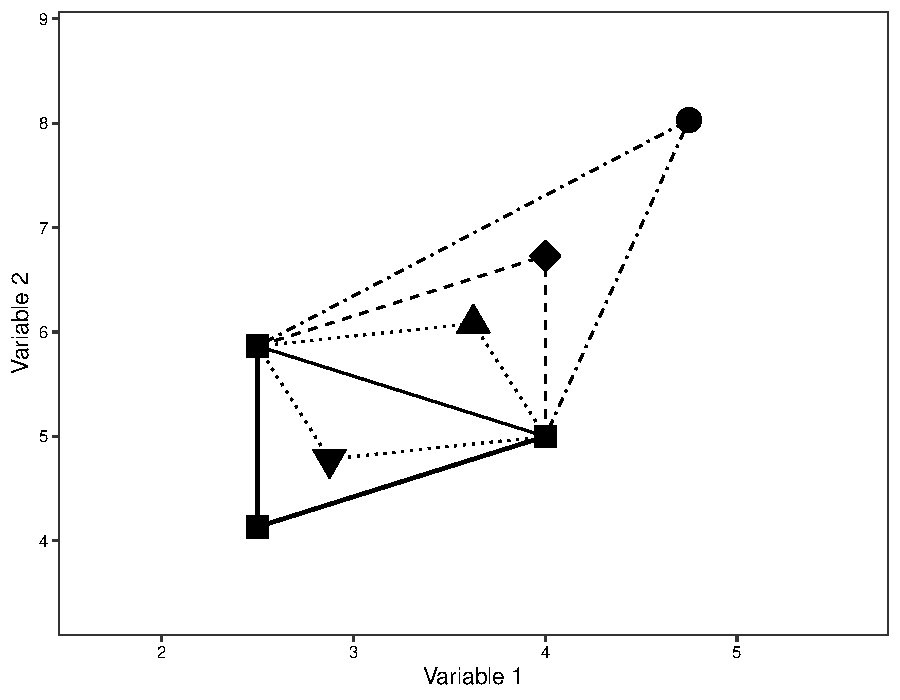
\includegraphics[width=0.6\textwidth]{chap2/images/simplexmov.pdf}
    \caption[Posibles movimientos de un símplex en un espacio bidimensional.]{Posibles movimientos de un símplex en un espacio bidimensional. Símplex original (\protect\squareblck), reflexión (\protect\squarerttdblck), expansión (\protect\circleblck), contracción del lado de la reflexión (\protect\triangleupblck) y contracción del lado del peor vértice (\protect\triangledownblck).}
    \label{fig:Simplexmov}
\end{figure}

Una de las ventajas más remarcables del algoritmo de optimización símplex es que el número de experimentos a realizar no crece de manera abrupta cuando se decide incluir más variables en el estudio. Por ejemplo, si en un diseño factorial a dos niveles se decide evaluar cuatro variables en lugar de tres, el número de experimentos de la matriz de diseño cambia de 8 a 16. Para la evaluación del simplex inicial, el número de experimentos cambia de cuatro a cinco. Esto hace menos importante el cribado de variables importantes que se recomienda antes del desarrollo de un diseño experimental más complejo.% (e.g.\ Matriz de Doehlert \citep{FERREIRA2004}).

El detalle de las reglas que gobiernan los algoritmos de optimización símplex y símplex modificado se describen con claridad en los capítulos tercero y cuarto del libro de \citet{simplexbook}. Ambos algoritmos han sido implementados en un paquete del lenguaje de programación \verb|R|. El paquete \verb|labsimplex| se encuentra disponible en de CRAN, y provee de herramientas para diseñar el símplex inicial, generar los vértices nuevos, visualizar gráficamente los movimientos del símplex y la evolución en la respuesta, entre otras cosas \citep{labsimplex}.


\section{Resumen}
En este capítulo se ha continuado con la exposición del litio como un elemento estratégico que es fundamental para la evolución de varias tecnologías que se proyectan a invadir el mundo, o que ya son ubicuas desde hace varios años. Se mencionaron aspectos relevantes de sus aplicaciones y de su contexto geopolítico. Se habló de las metodologías industriales que permiten su separación a partir de distintas fuentes naturales, y se hizo un resumen de algunas técnicas que se encuentran actualmente en desarrollo y que podrían ofrecer una alternativa para los procesos de extracción aplicados actualmente.

Las técnicas de separación cuyos conceptos son extrapolables a las \ac{PIM}s han sido descritas, y se han introducido los aspectos más importantes de la técnica aplicada en el presente trabajo. Se habló de las generalidades de las \ac{PIM}s y de los parámetros de transporte más importantes que caracterizan un sistema.

Finalmente se ha hablado de diseño de experimentos como la rama de la ciencia que está disponible para servir a todas las demás, haciendo más eficiente el trabajo en el laboratorio, y más robustas las conclusiones que pueden obtenerse a partir de los resultados disponibles.

\clearpage
\ChapBib{chap2/background}